%%%% ANEXO (B; ELEMENTO OPCIONAL)
%%
%% Texto ou documento não elaborado pelo autor, que serve de fundamentação,
%% comprovação e ilustração.

%% Locais (pastas) de ilustrações deste capítulo
\graphicspath{%
  {./Post-Textual/}%% Primário
  {./Post-Textual/Illustrations/}%% Secundário (descomentar se houver)
}

\chapter{Exemplos de Figura e Gráfico Produzidos em Aplicativos Específicos}%
\label{chpt:anx-b}

Figuras podem ser produzidas ou editadas com editores gráficos capazes de exportar a mesma em \ifbool{MakeAcr}{\intldescr{PS} (\intl{PS})}{\ENLang{PostScript} (PS)} ou, preferencialmente, \ifbool{MakeAcr}{\intl{EPS}}{EPS}.
O editor \href{https://www.xfig.org/}{Xfig\LinkIcon} é adequado para a maioria dos casos, mas outras opções para produção ou edição de diversas ilustrações são: \href{https://www.gimp.org/}{\ifbool{MakeAcr}{\intldescr{GIMP} (\intldescr+{GIMP} \textemdash\ \intl{GIMP})}{Programa de Manipulação de Imagem GNU (\ENLang*{GNU Image Manipulation Program} \textemdash\ GIMP)}\LinkIcon} e \href{http://dia-installer.de/}{Dia\LinkIcon}.
Este último é um editor orientado a diagramas (\ifbool{MakeAcr}{\intldescr{UML}\footnote{\IntlDescr+{UML} (\intl{UML})}}{Linguagem de Modelagem Unificada\footnote{\ENLang*{Unified Modeling Language} (UML)}}, fluxograma, etc.) com capacidade de exportar para diversos formatos, como na \Cref{fig:ex-uml} em \ifbool{MakeAcr}{\intl{PNG}}{PNG}~\cite{Larsson2020}.
Figuras em outros formatos (\ifbool{MakeAcr}{\intl{BMP}\footnote{\intldescr{BMP} (\intldescr+{BMP})}, \intl{GIF}\footnote{\intldescr{GIF} (\intldescr+{GIF})} e \intl{JPEG}}{BMP\footnote{Mapa de Bits (\ENLang*{Bitmap})}, GIF\footnote{Formato de Intercâmbio de Gráficos (\ENLang*{Graphics Interchange Format})} e JPEG}) podem ser convertidas para \ifbool{MakeAcr}{\intl{EPS}}{EPS} usando o aplicativo \href{https://github.com/jasper-software/xv.git}{XV\LinkIcon}, entre outros.
Este aplicativo não lista o \ifbool{MakeAcr}{\intl{EPS}}{EPS} dentre aqueles que consegue manipular, mas selecionando-se o \ifbool{MakeAcr}{\intl{PS}}{PS} e fornecendo-se a extensão \texttt{eps} ao nome do arquivo, o \ifbool{MakeAcr}{\intl{EPS}}{EPS} é produzido.

\begin{figure}[!htbp]
\SetCaptionWidth{\textwidth}
\caption[%
  Outro exemplo de figura (UML), produzida no editor gráfico Dia%
]{%
  Outro exemplo de figura (\ifbool{MakeAcr}{\intl{UML}}{UML}), produzida no editor gráfico \href{http://dia-installer.de/}{Dia\LinkIcon}%
}%
\label{fig:ex-uml}
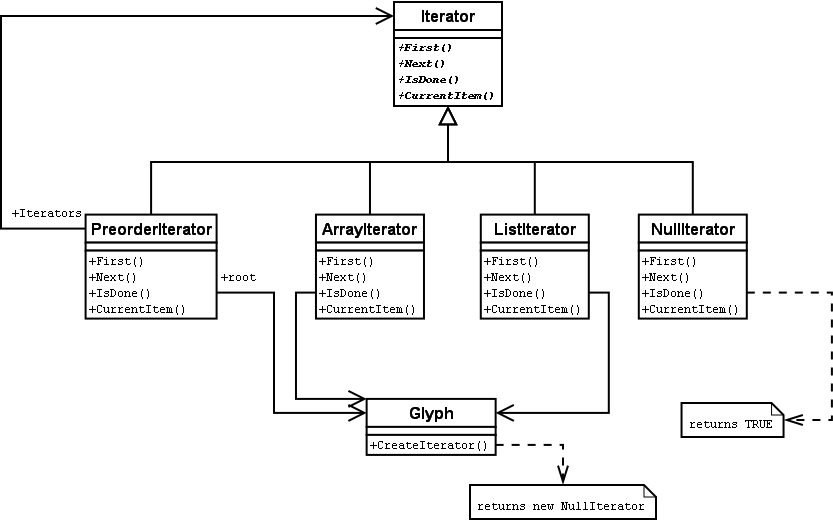
\includegraphics[width = \CaptionWidth]{fig-ex-uml}
\SourceOrNote{\textcite{Larsson2020}}
\end{figure}

Gráficos são produzidos com aplicativos capazes de exportar nos formatos \ifbool{MakeAcr}{\intl{PS} ou \intl{EPS}}{PS ou EPS}.
A ferramenta \href{http://www.gnuplot.info/}{gnuplot\LinkIcon} é uma das mais usadas para isto.
Uma vez no formato \ifbool{MakeAcr}{\intl{EPS}}{EPS}, gráficos são inseridos no texto, tal como figuras (ver \Cref{grph:ex-gnuplot}).

\begin{graph}[!htbp]
\SetCaptionWidth{0.7\textwidth}
\begin{minipage}{\CaptionWidth}
\caption[%
  Outro exemplo de gráfico, produzido em gnuplot a partir de arquivo de \ENLang*{script}%
]{%
  Outro exemplo de gráfico, produzido em gnuplot a partir de arquivo de \ENLang*{script}\footnote{\texttt{grph-ex-gnuplot.plt} em \texttt{./Post-Textual/Illustrations/}.}%
}%
\label{grph:ex-gnuplot}
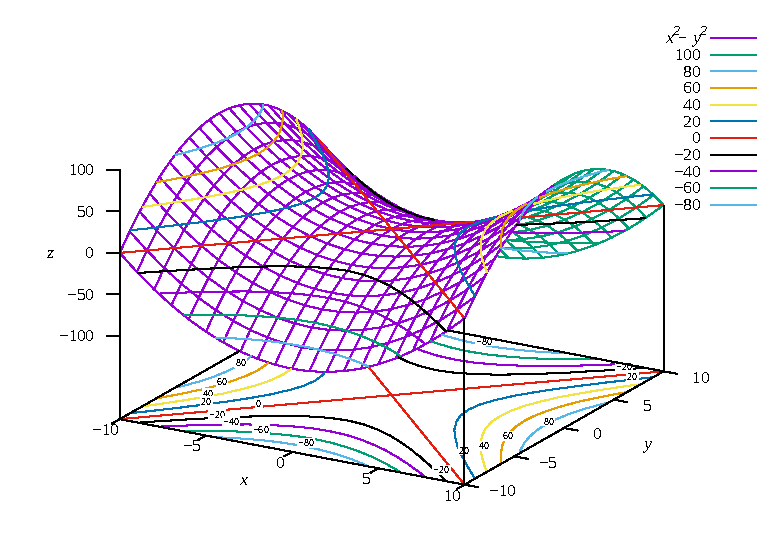
\includegraphics[width = \CaptionWidth]{grph-ex-gnuplot}
\end{minipage}
\SourceOrNote{adaptado de \textcite{Gnuplot2023}}
\end{graph}

\section{Título de seção secundária de anexo}%
\label{sect:anx-b2}

Exemplo de seção secundária de anexo (\Cref{sect:anx-b2}).

\subsection{Título de seção terciária de anexo}%
\label{ssect:anx-b3}

Exemplo de seção terciária de anexo (\Cref{ssect:anx-b3}).

\subsubsection{Título de seção quaternária de anexo}%
\label{sssect:anx-b4}

Exemplo de seção quaternária de anexo (\Cref{sssect:anx-b4}).

\paragraph{Título de seção quinária de anexo}%
\label{prgh:anx-b5}

Exemplo de seção quinária de anexo (\Cref{prgh:anx-b5}).

\subparagraph{Título de parágrafo (divisão de seção quinária) de anexo}%
\label{sprgh:anx-b6}

exemplo de parágrafo (divisão de seção quinária) de anexo (\Cref{sprgh:anx-b6}).
